\section{Feasibility Region}
\label{section_reasibility_region}

We aim to determine the set \highlight{$\mathcal{D}$} of points \highlight{$x[k] \in \mathcal{X}$} for 
which there exists \highlight{$\mathbf{\hat{u}[k]} \in \mathbb{R}^{pN}$} satisfying the constraints

\noindent
\begin{equation}
    \left[
    \begin{matrix}
        \mathbf{S_x} \mathbf{B} \\
        \mathbf{S_u} \\
    \end{matrix}
    \right] \mathbf{u} \le
    \left[
    \begin{matrix}
        \mathbf{b_x} - \mathbf{Sx} \mathbf{A} x[k] \\
        \mathbf{b_u}
    \end{matrix}
    \right]
\end{equation}

These restrictions can be rewritten as

\noindent
\begin{equation}
    \left[
    \begin{matrix}
        \mathbf{S_x} \mathbf{B} & \mathbf{S_x} \mathbf{A} \\
        \mathbf{S_u} & 0 \\
    \end{matrix}
    \right] 
    \left[
        \begin{matrix}
            \mathbf{u} \\
            x(0)
        \end{matrix}
    \right]
    \le
    \left[
    \begin{matrix}
        \mathbf{b_x} \\
        \mathbf{b_u}
    \end{matrix}
    \right]
\end{equation}

\noindent
adding a restriction \highlight{$S_x x(0) \le b_x$}

\noindent
\begin{equation}
    \left[
    \begin{matrix}
        \mathbf{S_x} \mathbf{B} & \mathbf{S_x} \mathbf{A} \\
        \mathbf{S_u} & 0 \\
        0 & S_x
    \end{matrix}
    \right] 
    \left[
        \begin{matrix}
            \mathbf{u} \\
            x(0)
        \end{matrix}
    \right]
    \le
    \left[
    \begin{matrix}
        \mathbf{b_x} \\
        \mathbf{b_u} \\
        b_x
    \end{matrix}
    \right]
\end{equation}

This can be written in a shorter form

\noindent
\begin{equation}
    S_w w \le b_w
\end{equation}

\noindent
with

\noindent
\begin{equation}
    w = 
    \left[
        \begin{matrix}
            \mathbf{u} \\
            x(0)
        \end{matrix}
    \right],
    S_w = 
    \left[
        \begin{matrix}
            \mathbf{S_x} \mathbf{B} & \mathbf{S_x} \mathbf{A} \\
            \mathbf{S_u} & 0 \\
            0 & S_x
        \end{matrix}
    \right],
    b_w = 
    \left[
        \begin{matrix}
            \mathbf{b_x} \\
            \mathbf{b_u} \\
            b_x \\
        \end{matrix}
    \right]
\end{equation}

The constraint \highlight{$S_w w \le b_w$} define a polyhedron \highlight{$\mathcal{P}_w$} 
in the space \highlight{$\mathbb{R}^{(pN+n)}$} corresponding to the variables \highlight{$\mathbf{u}$}, \highlight{$x(0)$}.

The set \highlight{$\mathcal{D}$} is obtained by projection \highlight{$\mathcal{P}_w$} onto the subspace of its last \highlight{$n$} components.

\comentariored{
    acertar a notacao nos eixos
}

\begin{figure}[h]
    \centering
    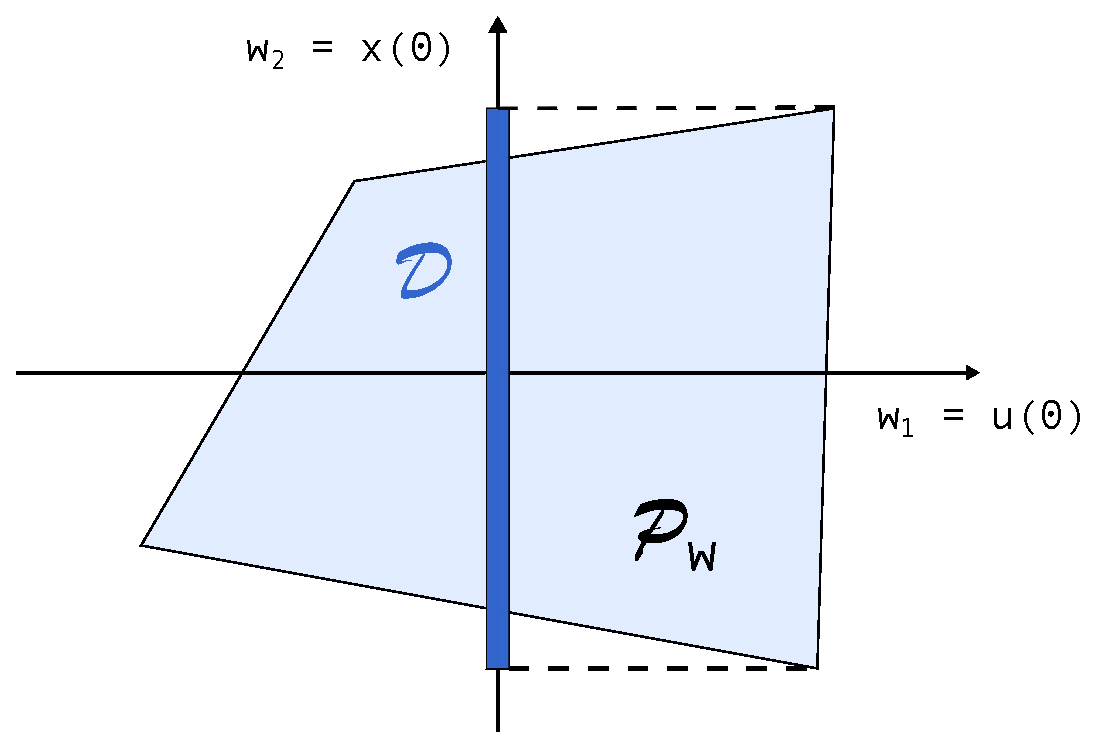
\includegraphics[width=0.7\textwidth]{Cap3/fig/feasability.eps}
    \caption{Illustration for n = 1 state, p = 1 input and N = 1 step}\label{cap3_feasability}
\end{figure}

The \textbf{projection} can be performed using the \textit{projection} function from the \textit{MPT Toolbox}.
